\documentclass[usletter,11pt,english,openany]{article}

%Primary packages
\usepackage{fancyvrb}

\usepackage[utf8]{inputenc}
\usepackage[english]{babel}
\usepackage[pdftex]{graphicx}


% Useful packages:

% Advanced mathematical formulas and symbols
% -------------------------------------
\usepackage{amsmath}
\usepackage{amssymb}
\usepackage{amsfonts}
\usepackage{bm}

% Footnotes
% -------------------------------------
\usepackage[stable,splitrule]{footmisc}

% Color management package
% -------------------------------------
\usepackage[usenames,dvipsnames]{xcolor}

% Control line spacing 
% -------------------------------------
% putting this between footmisc and hyperref seemed to fix broken footnote links
\usepackage{setspace}
\AtBeginDocument{\let~=\nobreakspace}
\spacing{1.1}

% Advanced crossreferencing commands 
% -------------------------------------
% Default settings:
% \usepackage[]{hyperref}
% Disable link coloring:
% \usepackage[colorlinks=false]{hyperref}
% Enable link coloring with personalized colors, make page number (not text) be link on the Table Of Contents (needs color package)
\PassOptionsToPackage{hyphens}{url} %for url linebreaks
\usepackage[colorlinks=true, linkcolor=BlueViolet, citecolor=BlueViolet, urlcolor=BlueViolet,linktocpage=true]{hyperref}

%% more footnote stuff
\usepackage{footnotebackref}

\let\oldFootnote\footnote
\newcommand\nextToken\relax

\renewcommand\footnote[1]{%
    \oldFootnote{#1}\futurelet\nextToken\isFootnote}

\newcommand\isFootnote{%
    \ifx\footnote\nextToken\textsuperscript{,}\fi}
    
% note for tables (with tabularx): if all table footnotes can't fit on the same page as the table, then they will all be shoved to the next page (seems like a bug); solution: use '\newpage' to put the table on a new page so footnotes fit (won't work if there are just too many footnotes)


% Flexible interface to page dimensions
% -------------------------------------
% Default settings:
% \usepackage[]{geometry}
% Set specific margins:
\usepackage{marginnote}
\usepackage[outer=2.62cm,inner=2.62cm,top=3cm,bottom=2.75cm, marginparwidth=2.1cm, marginparsep=.35cm]{geometry}


%Tree drawing
\usepackage{tikz}
\usetikzlibrary{trees, arrows}
\usepackage{pgfplots}
\pgfplotsset{compat=1.15}

\usepackage[edges,linguistics]{forest}


% Tabular package extensions
% -------------------------------------
% \usepackage{array}
% \usepackage{multirow}

% Modify chapter level headings
% -------------------------------------
\usepackage[Sonny]{fncychap}
\usepackage{fancyhdr}
\fancyhead{}
\fancyfoot{}
\rhead[\small \leftmark]{\small \thepage}
\lhead[\small \thepage]{\small \leftmark}
\setlength{\headheight}{13.2pt}

\ChRuleWidth{1pt}
\ChNameAsIs
\ChNameUpperCase
\ChNameVar{\Large\bf}
\ChNumVar{\Huge} 
\ChTitleVar{\LARGE}

% Modify appendix and add subappendices environments
% -------------------------------------
\usepackage{appendix}

% Paragraph indentation and skip
% -------------------------------------
\setlength{\parindent}{0pt}
\setlength{\parskip}{1.7ex plus 0.5ex minus 0.8ex}

\usepackage{xspace}
\newcommand\nd{\textsuperscript{nd}\xspace}
\newcommand\rd{\textsuperscript{rd}\xspace}
\newcommand\rds{\textsuperscript{rds}\xspace}
\newcommand\nth{\textsuperscript{th}\xspace}
\newcommand\nths{\textsuperscript{ths}\xspace}

% List spacing
\usepackage{enumitem}
\setlist[itemize]{topsep=0pt}
\newcommand{\listspace}{-.4em}

% Separate document into parts
\usepackage{titlesec}

% Copyright and Restricted tags
\usepackage{textcomp}
%$^{\tiny{\textregistered}}$
%$^{\tiny{\textcopyright}}$

% Advanced tables
\usepackage{ltablex}
\usepackage{ragged2e}

% add tabularx column type to prevent bad spacing when text wraps in a cell
\newcolumntype{R}{>{\RaggedRight\arraybackslash}X}

% Figure and Table reference numbering to be ChapterNum-FigNum
% Doesn't work for trees (yet?) so trees should be called Trees/Diagrams instead of Figures
\renewcommand\thetable{\thesection-\arabic{table}}
\renewcommand\thefigure{\thesection-\arabic{figure}}

% captions for figures
\usepackage[labelfont=bf]{caption}

% Line numbering for drafts only
%\usepackage[pagewise,modulo,displaymath,mathlines]{lineno}
%\linenumbers

% ___________________________________________________________________________________________________________
%
%                  		PDF INFO
% ___________________________________________________________________________________________________________




\hypersetup{
    pdftitle = {Seraphis}
}


\title{Seraphis: A Privacy-Preserving Transaction Protocol Abstraction (WIP)\footnote{\textbf{License}: Seraphis is released into the public domain.}\\\vspace{.3cm}
\large Draft v0.0.16\footnote{This is just a draft, so it may not always be available wherever it is currently hosted.}\vspace{-.715cm}}
\author{koe\footnote{Author `koe' worked on this document partly as an employee of MobileCoin, Inc.} \texttt{ ukoe@protonmail.com}}
\date{\vspace{-.5cm}\today\vspace{-1cm}}


\begin{document}
% ------ Title page ------------------------
\setlength{\abovedisplayskip}{0pt}
\setlength{\belowdisplayskip}{0pt}
\setlength{\abovedisplayshortskip}{0pt}
\setlength{\belowdisplayshortskip}{0pt}

%\pagenumbering{roman}
%\pagestyle{plain}
%\thispagestyle{empty}

\pagenumbering{arabic}
\pagestyle{fancy}

\maketitle

% ___________________________________________________________________________________________________________
%
%             			CONTENT
% ___________________________________________________________________________________________________________

%\newpage

% -------- Chapters ----------------------------

%\section{Abstract}
%\label{sec:abstract}
\begin{abstract}
    Seraphis\footnote{The name `Seraphis' is derived from Serapis, a Graeco-Egyptian syncretistic deity. Syncretism is the combination/reconciliation of different ideas/ways of thinking, similar to how Seraphis is a protocol that brings together many ideas and permits a variety of proving systems.} is a privacy-focused transaction protocol abstraction for p2p electronic cash systems. Seraphis transaction outputs, called {\em e-notes} in this paper, are amount-transfer devices in the RingCT tradition, which record an `amount' as a Pedersen commitment and an `address with transfer-authority' as a specially-designed prime-order group point (similar to CryptoNote one-time addresses). Unlike previous protocols compatible with Confidential Transactions (CT), where enote membership, ownership, and unspentness proofs were highly integrated into one large proving structure (such as MLSAG or CLSAG in the case of standard RingCT), Seraphis separates membership proofs from ownership and unspentness proofs. This greatly simplifies the requirements for membership proofs, allowing more efficient proving structures to be used. Doing so also allows a linking tag (a.k.a.\ key image) construction with a number of favorable properties. Most notably, it is possible to have a Seraphis-compatible addressing scheme which permits wallets with three tiers of permissions (view received amounts, full balance recovery, full balance recovery with spend authority). The second permission tier is unique to Seraphis among protocols in the CryptoNote tradition.\footnote{An example of such a scheme is discussed in this paper's companion paper [citation TBD].}
\end{abstract}


\section{Introduction}
\label{sec:introduction}

A p2p (peer-to-peer) electronic cash system is a monetary system where the entire supply of currency exists as a set of digital records describing money amounts and their owners. Those records can be stored by any person, and transactions (attempts to transfer money to new owners) are mediated by a network of {\em peers} (usually called {\em nodes}). Such systems are typically designed with the goal that no participant in the system has the power to easily censor transactions, re-spend funds that have been spent before, or increase the total money supply at will.

To achieve that goal, it is necessary for such systems to be decentralized. The peers who mediate transactions (checking their validity with respect to the existing state of the money supply, and deciding which of N conflicting transactions to accept) do not necessarily trust each other. It is therefore beneficial to have a common rule-set and format for constructing transactions, so that any peer can validate any transaction and reach consensus with other peers/nodes about changes to the recorded monetary state. The transaction rule-set and format used by any given p2p electronic cash system is called its {\em transaction protocol}.

Seraphis is a transaction protocol {\em abstraction}, which means it defines the rule-set that a transaction protocol must satisfy (and the corresponding security model) without specifying any concrete proving systems or semantic constraints.


\subsection{Monetary state}
\label{subsec:intro-monetary-state}

Most modern p2p electronic cash systems are `cryptocurrencies' in the tradition of Bitcoin~\cite{Nakamoto_bitcoin}. In Bitcoin, each (archival) node maintains a full copy of all mutations to the monetary state that led from Bitcoin's inception up to the current moment (called a {\em ledger}).

The monetary state of a cryptocurrency arises from all the `money creation' and `amount transfer' events that have occurred since the currency was born. Almost universally, those events are defined in the {\em transaction output} model (henceforth called the {\em enote} model). An enote is a small message containing an `amount' of money, an `ownership address' that encapsulates the authority to spend the enote, and an optional arbitrary memo.

\begin{itemize}
    \item \textbf{Money creation event}: Create a new `coinbase enote', which increases the total supply of money.
    \item \textbf{Money transfer event (transaction)}: Consume one or more previously unspent enotes to transfer the amounts they record to one or more new enotes (see Section \ref{sec:seraphis}).
\end{itemize}

The `current monetary state' of a cryptocurrency is therefore the set of spent and unspent enotes recorded in the ledger.


\subsection{Transaction protocols}
\label{subsec:intro-transaction protocols}

Transaction protocols must always codify a basic set of rules.

\begin{itemize}
    \item \textbf{Membership}: enotes spent by a transaction must already exist in the ledger.
    \item \textbf{Unspentness}: enotes spent by a transaction must be unspent prior to that transaction.
    \item \textbf{Ownership}: A transaction author must have the authority to spend the transaction's input enotes.
    \item \textbf{Amount balance}: The total amount in enotes spent by a transaction must equal the total amount in new enotes created (plus a transaction fee, usually).
\end{itemize}

A very simple transaction protocol could implement those rules like this:

\begin{itemize}
    \item \textbf{Membership}: Reference existing enotes with their indices in the ledger. Transaction validators can look up those enotes directly.
    \item \textbf{Unspentness}: When an enote is spent by a transaction, set a bit flag next to that enote in the ledger. Reject transactions that reference spent enotes.
    \item \textbf{Ownership}: Define ownership with public key cryptography. Let each enote's address record a public key specified in advance by the intended owner. To spend an enote, its owner must create a cryptographic signature with the address key and add the signature to their transaction.\footnote{The `crypto' in `cryptocurrency' refers to the use of cryptography to control enote ownership.}
    \item \textbf{Amount balance}: Record enote amounts in clear text and use simple sums to check that input amounts equal output amounts (disallowing integer overflow).
\end{itemize}

An unfortunate consequence of cryptocurrencies being decentralized is that the ledger is `public'. This means all enotes and transaction events are public knowledge. If amounts are in cleartext, addresses can be reused, and enotes to be spent are referenced directly, then observers can discern many details about users' finances.

A lack of privacy in the design of a transaction protocol has two main drawbacks, which lead to a competitive disadvantage versus protocols that include elements of privacy (all else being equal).

\begin{enumerate}
    \item Privacy is valuable to real people. Typically, it is preferable to choose when others obtain information about you than for that information to be available automatically.
    \item Fungibility and privacy go hand-in-hand. If observers have detailed information about the ledger, then it is possible for some enotes to be more valuable than other enotes just based on differences in who owns them or where they originated (i.e.\ the history/transaction-graph that led to those enotes being created), even if the amounts they contain are the same.
\end{enumerate}

We believe an ideal transaction protocol should satisfy the following informal privacy matrix.

\begin{itemize}
    \item \textbf{Recipients}
    \begin{itemize}
        \item \textbf{Know}: Amounts received, and when they were received.
        \item \textbf{Don't know}: Who sent them any given amount.
    \end{itemize}
    \item \textbf{Senders}
    \begin{itemize}
        \item \textbf{Know}: Amounts sent, when they were sent, and who they were sent to.\footnote{A transaction author inherently knows who they send enotes to. This information does not need to be stored in the ledger to satisfy this privacy matrix.}
        \item \textbf{Don't know}: If an amount sent to someone else has been spent.
    \end{itemize}
    \item \textbf{Observers}
    \begin{itemize}
        \item \textbf{Know}: The number of inputs/outputs in each transaction, fees paid by each transaction, and when each transaction was added to the ledger.
        \item \textbf{Don't know}: The amounts involved in any transaction (other than fees), the relationships between any transactions, or the amounts owned by any user.
    \end{itemize}
\end{itemize}

Most of these requirements are relatively easily met by CryptoNote-style addressing and linking tags (a.k.a.\ key images) \cite{cryptoNoteWhitePaper} and Confidential Transactions \cite{maxwell-ct-2}, which were first combined in the protocol RingCT \cite{MRL-0005-ringct}. There are two areas of weakness in existing protocols based off RingCT.

\begin{itemize}
    \item Observers can, to some extent, discern when a transaction was constructed, which is stronger information than simply `when a transaction was added to the ledger'. The biggest culprit for this lies in transaction fees, which are often a function of real-world time. The problem of transaction timing is out of scope for this paper.
    \item Observers can, to some extent, discern relationships between transactions. Membership proofs defined in RingCT (and those used in related protocols like Triptych \cite{triptych-preprint}, Lelantus-Spark \cite{lelantus-spark}, Omniring \cite{omniring-paper}, and RingCT3.0 \cite{ringct3-preprint}) have `anonymity sets'. A transaction author proves that each enote spent by their transaction exists in a small set of enotes, and further proves that that small set is a subset of enotes that exist in the ledger. Unfortunately, if observers see that one transaction references an enote created by another transaction, then they know there is more likely to be a relationship between those transactions than if no such connection exists. This probabilistic knowledge is stronger than the `pure/ideal' case where a membership proof shows that an enote exists in the ledger without giving any hints about which one it might be.
\end{itemize}

Increasing the anonymity set size of membership proofs naturally reduces how much information observers can glean from transactions. However, combining membership proofs with ownership and unspentness proofs in one large proving structure, a ubiquitous pattern in previous RingCT-inspired protocols, has led to some challenges around increasing that size.

Most importantly, proving structures suitable for both membership proofs and ownership/unspentness proofs place constraints on the construction of linking tags, which are the core element of unspentness proofs in privacy-focused transaction protocols. A linking tag is an `image' of an enote's address produced when trying to spend the enote. If a transaction's input proofs contain a linking tag that already exists in the ledger, then the transaction is trying to re-spend an enote that has already been spent.

As one example of those constraints, the transaction protocol Triptych \cite{triptych-preprint}, which allows a proving structure an order of magnitude more efficient than those allowed by standard RingCT, features a linking tag construction that looks like $\tilde{K} = (1/k^o)*U$. Here $k^o$ is the private key of the address that owns a given enote, and $U$ is a generator of a prime-order cyclic group. By inverting $k^o$ to create linking tags, it becomes relatively more difficult to design a multisignature scheme where multiple individuals collaborate to sign transactions, compared to a construction that is linear in $k^o$. This is because a linear construction would allow a simple sum of components provided by signature participants (such as in \cite{MRL-0009-multisig}), whereas an inverted shared key requires a non-trivial signing protocol (e.g.\ involving Paillier encryption \cite{inversion-style-multisig-mrl-72}).


\subsection{Our contribution}
\label{subsec:intro-our-contribution}

The main innovation of Seraphis compared to its predecessors is separating ownership and unspentness proofs from membership proofs. Seraphis membership proofs only say (more-or-less) that a commitment to an enote corresponds with an enote in some reference set. The prover then operates on the enote commitment to demonstrate ownership and unspentness and to connect it with the proof that amounts balance.

This separation allows the definition of linking tags to be fairly open-ended. We designed a linking tag construction with the following (informal) properties.

\begin{enumerate}
    \item \textbf{Multisig compatibility}: Linking tags are composed of two pieces of private key material associated with an enote's address. One piece is transformed linearly from the address to the tag, while the other piece is inverted (see Section \ref{subsec:seraphis-ownership-unspentness-proofs}).

    A multisignature group may share knowledge of the inverted component and split knowledge of the linear component. This facilities straightforward multisignature schemes for ownership and unspentness proofs.

    \item \textbf{Address scheme flexibility}: The linking tag construction makes it is possible to implement user addressing schemes with multiple tiers of permissions (see this paper's companion paper [citation TBD]). Most significantly, it is possible to have a `view entire balance' tier that is fully separated from the `spend authority' tier.
\end{enumerate}

In Appendix \ref{appendix:squashed-enote-model} we introduce a more-restrictive membership proof model layered on the primary model in this paper. We call it the `squashed enote' model. Concrete proving structures in that model are non-trivially more efficient than structures in the plain model, allowing relatively larger anonymity set sizes as a function of proof complexity and size compared to structures in the plain model, when comparing structures based on the same proving systems (see an efficiency analysis in Section \ref{sec:efficiency}).

Appendix \ref{appendix:composition-with-schnorr} introduces Seraphis composition proofs, which are a Seraphis-compatible ownership/unspentness proof. Appendix \ref{appendix:grootle-proof} introduces Grootle proofs, a Seraphis-compatible membership proof for the squashed enote model.



\subsection{Acknowledgements}
\label{subsec:intro-acknowledgements}

We would like to thank Aaron Feickert and Aram Jivanyan (who wrote Lelantus-Spark \cite{lelantus-spark}, a transaction protocol very similar to Seraphis) for critical discussions that led to Seraphis's linking tag construction, and Nikolas Kr{\"{a}}tzschmar for pointing out a flaw in an earlier version of that construction.



\section{Preliminaries}
\label{sec:preliminaries}

\subsection{Public parameters}
\label{subsec:preliminaries-public-parameters}

\footnote{This section was copied mostly verbatim from the Triptych preprint \cite{triptych-preprint}.}Let $\mathbb{G}$ be a cyclic group of prime order $l > 3$ in which the discrete logarithm problem is hard and the decisional and inverse decisional Diffie-Hellman assumptions hold, and let $\mathbb{Z}_l$ be its scalar field. Let $\mathcal{H}: [0,1]^* \to \mathbb{Z}_l$ be a cryptographic hash function. We add a subscript to $\mathcal{H}$, such as $\mathcal{H}_1$, in lieu of domain-separating the hash function explicitly; any domain-separation method may be used in practice (e.g.\ an ASCII string corresponding to a domain-separated use case, such as $\mathcal{H}(``sender\_receiver\_secret"\ ||\ [\textrm{hash input}])$).

Let each of the following sets contain generators of $\mathbb{G}$, where each generator's discrete logarithm with respect to other generators in the same set is unknown (there may be intersections between sets): $\{G_0, G_1,...,G_n\}$, $\{H_0, H_1,...,H_m\}$, and $\{J\}$ (for arbitrary integers $n$, $m$). Note that all such generators may be produced using public randomness. For example, the use of a hash function with domain separation may be appropriate. All public parameters are assumed to comprise a global reference string known to all players. For readability, we generally exclude explicit reference to public parameters in algorithm definitions and Fiat-Shamir transcript hashes.


\subsection{Notation}
\label{subsec:preliminaries-notation}

\begin{itemize}
    \item We use additive notation for group operations on $\mathbb{G}$. This means, for example, that the binary group operation between $G$ and $H$ is denoted $G + H$.

    \item This paper contains no exponentiation outside Appendix \ref{appendix:grootle-proof}. Superscripts, such as the $o$ in $k^o$, are merely for descriptive purposes and have no mathematical significance.

    \item For group element $P$ and scalar $x \in \mathbb{Z}_l$, $x P$ and $x*P$ both indicate scalar multiplication. The use of asterisks ($*$) in some places but not others is meant to aid visual clarity where appropriate (usually when multiplying by a parenthesized scalar or by a scalar that has a superscript).

    \item Modular multiplicative inverse group operations use the notation $(1/x)*P$.

    \item Tuples are indicated with brackets, e.g.\ $[A, B, C]$. To avoid confusion, we always explicitly refer to tuples as tuples wherever they appear (e.g.\ `the tuple $[A, B, C]$').
\end{itemize}



\section{Seraphis}
\label{sec:seraphis}

In this section we discuss the various components of Seraphis, with security theorems and proofs introduced where appropriate [[[TODO]]]. Seraphis is an {\em abstract} protocol, so various implementation details are left undefined. An implementer needs to define the generators $G_0, G_1, G_2, H_0, H_1, J$, specify a membership proof structure (e.g.\ Appendix \ref{appendix:grootle-proof}), specify an ownership/unspentness proof structure (e.g.\ Appendix \ref{appendix:composition-with-schnorr}), define how to check that transaction amounts balance, define an address scheme, and define an information recovery scheme. See this paper's companion paper [citation TBD] for a complete instantiation of Seraphis.


\subsection{Transaction overview}
\label{subsec:seraphis-transaction-overview}

For context, we outline the content of a transaction here.

\begin{itemize}
    \item \textbf{Inputs}: A transaction spends old enotes.
    \begin{itemize}
        \item \textbf{Enote images}: Representations of the enotes spent by this transaction, including their linking tags (Section \ref{subsec:seraphis-enote-images}).
        \item \textbf{Membership proofs}: Proof structures demonstrating that each enote image is constructed properly from a real enote in the ledger (Section \ref{subsec:seraphis-membership proofs}).
        \item \textbf{Ownership and unspentness proofs}: Proof structures that use enote images to demonstrate ownership and unspentness for each spent enote (Section \ref{subsec:seraphis-ownership-unspentness-proofs}).
    \end{itemize}
    \item \textbf{Outputs}: A transaction creates new enotes.
    \begin{itemize}
        \item \textbf{Enotes}: New enotes (Section \ref{subsec:seraphis-enotes}). The total amount they contain equals the total amount in spent enotes (Section \ref{subsec:seraphis-amount-balance-proofs}).
        \item \textbf{Range proofs}: Proof structures demonstrating that amount commitments in new enotes are legitimate (part of the Confidential Transactions technique) (Section \ref{subsec:seraphis-amount-balance-proofs}).
    \end{itemize}
    \item \textbf{Balance proof}: A proof that the sum of input amounts equals the sum of output amounts (Section \ref{subsec:seraphis-amount-balance-proofs}).
    \item \textbf{Miscellaneous}: Miscellaneous other data included with a transaction, such as a transaction fee.
\end{itemize}


\subsection{Enotes}
\label{subsec:seraphis-enotes}

Seraphis enotes are composed of an amount commitment, an address, and a memo.

\begin{itemize}
    \item \textbf{Amount commitment}: A Pedersen commitment $C$ (with blinding factor $x$) to the amount $a$ contained in the enote \cite{Pedersen1992, maxwell-ct-2}.
    \[C = x H_0 + a H_1\]

    \item \textbf{Address}: A public key $K^o$ composed of three generators $G_0$, $G_1$, and $G_2$, and three corresponding private keys $k^o_0$, $k^o_1$, and $k^o_2$. The enote's owner must prove knowledge of those private keys if they want to transfer the amount $a$ to new enotes (it is allowed for $k^o_0$ to equal zero).\vspace{.115cm}
    \[K^o = k^o_0*G_0 + k^o_1*G_1 + k^o_2*G_2\]

    \item \textbf{Memo}: An arbitrary memo field. This usually includes information that helps the enote's owner identify that they own it, learn the private keys $k^o_i$, and reconstruct the amount commitment. See Sections \ref{subsec:seraphis-information-recovery} and \ref{subsec:implementers-information-recovery}.
\end{itemize}


\subsection{Enote images}
\label{subsec:seraphis-enote-images}

An enote image is a representation of an enote.

\begin{itemize}
    \item \textbf{Masked commitment}: The enote's commitment with an additional masking factor.\vspace{.115cm}
    \begin{align*}
        C' &= t_c H_0 + C \\
        C' &= (t_c + x)*H_0 + a H_1 \\
        C' &= v_c H_0 + a H_1
    \end{align*}

    \item \textbf{Masked address}: The enote's address with a masking factor.\vspace{.115cm}
    \begin{align*}
        K' &= t_k G_0 + K^o \\
        K' &= (t_k + k^o_0)*G_0 + k^o_1*G_1 + k^o_2*G_2
    \end{align*}

    \item \textbf{Linking tag}: The enote's linking tag.\vspace{.115cm}
    \[\tilde{K} = (k^o_2/k^o_1)*J\]
\end{itemize}

The blinding factors $t_c$ and $t_k$ must be statistically independent and selected at random from a uniform distribution. [[[formalize better?]]] Note that observers who don't know $t_c$ and $t_k$ cannot look at an enote image and discern what enote it was created from.

We describe how a transaction author can prove that enote image addresses and commitments are constructed properly from real enotes in Section \ref{subsec:seraphis-membership proofs}, and further prove that linking tags are constructed properly from enote image masked addresses in Section \ref{subsec:seraphis-ownership-unspentness-proofs}.

\subsubsection{Sender-receiver anonymity}
\label{subsubsec:enote-images-sender-receiver-anonymity}

If a person spends an enote, they should expect that the person who originally sent them that enote will not know it is spent.

If $t_c$ and $t_k$ are randomly selected and unknown to the original sender, then the sender cannot detect the original enote by inspecting the enote image's commitment and address.

We further argue in Sections \ref{subsec:seraphis-membership proofs}, \ref{subsec:seraphis-ownership-unspentness-proofs}, and \ref{subsec:seraphis-address-model} that input proofs and linking tags will not break sender-receiver anonymity.

\subsubsection{Linking tags}
\label{subsubsec:enote-images-linking-tags}

Linking tags are uniquely defined by the private keys $k^o_1$ and $k^o_2$ (as proven in Section \ref{subsec:seraphis-ownership-unspentness-proofs}). This means for a user to create two distinct linking tags from the same address, they must be able to solve one of the DLPs between generators $G_0$, $G_1$, and $G_2$, which we assume to be a hard problem [[[elaborate this proof?]]].

Since linking tags are assumed to be unique for each unique address $K^o$, they can be used to prove unspentness. If a transaction contains an enote image with a linking tag that has appeared in the ledger, then that transaction is invalid. The word `linking' refers to the ability of observers to link attempts to spend the same enote.

Note that if two enotes have the same address $K^o$, then only {\em one} of them can be spent, hence the superscript $o$. Going along with the CryptoNote tradition, $K^o$ can be referred to as a {\em one-time address}. The construction of one-time addresses is further discussed in Section \ref{subsec:seraphis-address-model}.


\subsection{Membership proofs}
\label{subsec:seraphis-membership proofs}

Every input to a transaction must have a membership proof. The proof must demonstrate that the input's enote image was built from an enote that exists in the ledger.

A proving system/structure is only eligible to be used as a Seraphis membership proof if it can satisfy the following abstract model. [[[formalize better?]]]

\begin{enumerate}
    \item Let $\mathbb{S}$ represent a set of tuples $[K_i, C_i]$, where\vspace{.115cm}
    \begin{align*}
        K_i &= z_i G_0 + s_{i,1} G_1 + s_{i,2} G_2 + ... + s_{i,n} G_n \\
        C_i &= x_i H_0 + a_{i,1} H_1 + a_{i,2} H_2 + ... + a_{i,m} H_m
    \end{align*}

    \item Let $\tilde{S}$ represent a tuple $[K', C']$, where\vspace{.115cm}
    \begin{align*}
        K' &= z' G_0 + s'_1 G_1 + s'_2 G_2 + ... + s'_n G_n \\
        C' &= x' H_0 + a'_1 H_1 + a'_2 H_2 + ... + a'_m H_m
    \end{align*}

    \item The proving system must be able to demonstrate that, within a security parameter $k$, $\tilde{S}$ corresponds to some $S_{\pi} \in \mathbb{S}$, where $\pi$ is unknown to the verifier, such that:
    \begin{enumerate}
        \item $s'_p == s_{\pi,p}$ for $p \in 1,...,n$
        \item $a'_q == a_{\pi,q}$ for $q \in 1,...,m$
    \end{enumerate}

    \item The proving system should be considered unusable if, given a proof $\sigma$ that $\tilde{S}$ corresponds to some $S_{\pi}$ in the set $\mathbb{S}$, an observer can guess the index $\pi$ with probability $> 1/|\mathbb{S}'| + \epsilon(k)$, where $\mathbb{S}' = \mathbb{S}$\textbackslash$\mathbb{S}_O$ and $S_{\pi} \in \mathbb{S}'$, $\mathbb{S}_O$ are tuples the observer knows can't have been subjects of the proof (in the context of Seraphis, if tuples $S$ represent enotes, then for example he owns the enotes in $\mathbb{S}_O$), and the observer has no special knowledge about the elements in $\mathbb{S}'$ (however, he can know $z_i G_0$, $x_i$, and $a_{i,q}$ for all $S_i \in \mathbb{S}'$).\footnote{In practice, $\pi$ can often be guessed with probability at least marginally above $1/|\mathbb{S}'|$. This is because the circumstances around when enotes are recorded in the ledger are often observable. Things like timing information, patterns of behavior, IP addresses of transaction submitters, transaction fees, etc., can all form the basis of heuristics for analyzing the true member referenced by a membership proof. See the discussions in \cite{AnalysisOfLinkability} and \cite{foundations-ring-sampling} for example.}
\end{enumerate}

In the context of Seraphis, we straightforwardly construct tuples $S$ directly from enotes, which can be referenced with simple ledger indices for verifiers to find (in a naive implementation),\footnote{If the size of $\mathbb{S}$ is small, then it may be practical to reference enotes with simple indices. As $\mathbb{S}$ gets large, more sophisticated data-compression techniques are advisable to minimize transaction sizes. For example, deterministically selecting members of the anonymity set using public entropy and a hash function \cite{chator-green-how-to-squeeze-crowd}.} and tuples $\tilde{S}$ from enote images. Readers will note that a membership proof says nothing about how $K$ and $C$ are constructed (i.e.\ the values of $G_0,...$, $H_0,...$, etc.). In future sections we will add more constraints to guarantee that enotes and enote images found in transactions have the expected forms (within a security parameter).

A trivial proof that satisfies the above model would be a pair of signatures on commitments to zero $K' - K = t_k G_0$ and $C' - C = t_c H_0$, given a reference set $\mathbb{S}$ that contains only one tuple $[K, C]$. More interesting solutions include a CSAG (a CLSAG \cite{clsag-eprint} without linking) on a ring of such commitment to zero pairs (assuming $G_0 == H_0$), a Groth/Bootle one-of-many proof \cite{groth-one-out-of-many, bootle-one-of-many, triptych-preprint, lelantus-spark} on a collection of those pairs, or a Groth/Bootle one-of-many proof applied to the squashed enote model (see Appendices \ref{appendix:squashed-enote-model} and \ref{appendix:grootle-proof}).


\subsection{Ownership and unspentness proofs}
\label{subsec:seraphis-ownership-unspentness-proofs}

Alongside each membership proof must be an ownership and unspentness proof. In Seraphis, `unspentness' is checked by looking for linking tag duplicates in the ledger. However, it is necessary to prove that linking tags are properly constructed. This is done simultaneously with the ownership proof to ensure the linking tag is derived from the relevant enote address.

A proof structure is only eligible to be used for Seraphis ownership/unspentness proofs if it can accomplish the following.

\begin{enumerate}
    \item Assume there is a group point $K = x G_0 + y G_1 + z G_2$.

    \item Demonstrate knowledge of values $x, y, z$ such that $K = x G_0 + y G_1 + z G_2$ and $y \neq 0, z/y \neq 0$.

    \item Demonstrate that a key $\tilde{K}$ satisfies $\tilde{K} == (z/y)*J$.

    \item A prover who knows $x$ and/or $y$, but not $z$, must be unable to create a proof that contains $\tilde{K} = (z/y)*J$ (within a security factor).
\end{enumerate}

%[[[CLARIFY LINKABILITY: two signatures should be linkable IFF $\tilde{K}$ is the same between them.]]] 
%[[[CLARIFY PRIVACY: an observer who knows all of $x, K, y G_1, z G_2$ should be unable to make the linking tag $\tilde{K}$ nor realize that it was produced from $K$ (assuming they don't have access to a proof demonstrating that).]]]

We integrate that `composition proof' model into Seraphis in the following way (see Appendix \ref{appendix:composition-with-schnorr} for an example proof structure that satisfies the model).

Suppose a membership proof $\sigma_{mp}$ shows that $\tilde{S}$ corresponds to some $S_{\pi}$ in the set $\mathbb{S}$. Then suppose the key $K' = z' G_0 + s'_1 G_1 + s'_2 G_2 + ...$ from $\tilde{S}$ is passed as input to the above proof system, and a valid proof is created. Observe the following.

\begin{itemize}
    \item For the composition proof to succeed, it must be the case that all $s'_p == 0$ for $p \geq 3$. This implies the key $K_{\pi}$ from $S_{\pi}$ (which $K'$ is based on) has the following form: $K_{\pi} = z_{\pi} G_0 + s_{\pi, 1} G_1 + s_{\pi, 2} G_2$. Moreover, the prover must know $z_{\pi}, s_{\pi, 1}, s_{\pi, 2}$.

    \item It must be the case that $\tilde{K} = (s_{\pi, 2}/ s_{\pi, 1})*J$.

    \item The verifier will not be able to discern which $S_i$ in the set $\mathbb{S}$ corresponds with $K'$.
\end{itemize}

Now suppose a transaction spends an enote. Let them set $S_{\pi} = [K^o_{\pi}, C_{\pi}]$ using the enote's one-time address and amount commitment, give $S_{\pi}$ a membership proof $\sigma_{mp}$, and give the resulting image $S' = [K', C']$ a composition proof $\sigma_{cp}$. With this proof pair, the verifier can be confident that the transaction author owns an enote in the set $\mathbb{S}$ (i.e.\ they know the keys $z_{\pi} = k^o_o$, $s_{\pi,1} = k^o_1$, and $s_{\pi,2} = k^o_2$ for some unknown index $\pi$), and that the linking tag $\tilde{K} = (k^o_2/k^o_1)*J$ in the composition proof is valid and can be used to check if the enote at index $\pi$ is unspent. Importantly, linking tag $\tilde{K}$ is independent of $z_{\pi}$ and $z'$ and hence is unaffected by the transformation from enote to enote image.

The transaction's enote image structure records $\tilde{S} = [K', C']$ and $\tilde{K}$ for observers/verifiers to reference (recall Section \ref{subsec:seraphis-enote-images}).


\subsection{Amount balance proofs}
\label{subsec:seraphis-amount-balance-proofs}

In accordance with the Confidential Transactions technique \cite{maxwell-ct-2}, Seraphis amounts are recorded as {\em Pedersen commitments}, which hide the amounts involved from observers (they have the `perfectly hiding' property). Even though observers cannot see transaction amounts directly, they should still be able to verify that the sum of input amounts always equals the sum of output amounts in every transaction.

First note that, thanks to our membership proof model (Section \ref{subsec:seraphis-membership proofs}), the commitment $C'$ in an enote image will contain the same values $a_{\pi,1},...,a_{\pi,m}$ as the commitment $C$ in the enote being spent. In Section \ref{subsubsec:confidential-transactions-range-proofs} we will prove that enote commitments have the form $C = x G_0 + a G_1$ as expected (i.e.\ prove that $a_{\pi,q} == 0$ for $q \geq 2$), and hence the amount $a$ in $C' = v_c G_0 + a G_1$ equals the amount in the original commitment.

Pedersen commitments have the `homomorphic' property, which means, for example, that if $P_1 = p_1 G$ and $P_2 = p_2 G$, then $P_1 + P_2 == (p_1 + p_2)*G$. We should therefore expect that if we sum together enote image commitments (inputs) and sum together new enote commitments (outputs), then $\sum C'_j - \sum C_t$ will contain no $H_1$ component only if the sum of input amounts equals the sum of output amounts.

An implementation of Seraphis must do the following.

\begin{enumerate}
    \item Demonstrate knowledge of the `remainder' $p_r$ in the commitment to zero $\sum C'_j - \sum C_t = p_r H_0$. It is acceptable if $p_r == 0$, such that $\sum C'_j == \sum C_t$ can be checked directly.
\end{enumerate}

\subsubsection{Range proofs}
\label{subsubsec:confidential-transactions-range-proofs}

Since Pedersen commitments are elements of a cyclic group, it is conceivable that the sum of amounts modulo the group order is less than the absolute sum of amounts.\footnote{For example, in a cyclic group of order 11, $7 + 7 \equiv 3 \pmod{11}$. If the input amount is 3, then the output amount could be 14!} To properly convince observers that transaction amounts balance, transaction authors must provide a `range proof' for each new enote's commitment.

A range proof must demonstrate the following for a given commitment $C = x H_0 + a H_1$.\footnote{At this time, Bulletproofs+ by Chung et.\ al \cite{bulletproofs_plus} (based on Bulletproofs by B\"{u}nz et.\ al \cite{Bulletproofs_paper}) is thought to be the most efficient zero-knowledge proving structure for range proofs, without a trusted setup.}[[[formalize this better?]]]

\begin{itemize}
    \item Prove knowledge of $x$ and $a$ such that $C = x H_0 + a H_1$.

    \item Show that the value $a$ is in the range $[0, 2^{z} - 1]$.
\end{itemize}

The maximum number of elements $n$ that can be summed together must be $n < l / (2^z - 1)$, otherwise range proofing those elements is pointless. Typically $z = 64$ and $l \approx 2^{252}$ (e.g.\ in Ed25519 \cite{Bernstein2012-high-speed-high-security-ed25519}), so $n$ can be as large as $\approx 2^{192}$. However, usually $n << 2^{64}$ for practical reasons.

In a real system based on Seraphis, only new enote commitments need range proofs, not enote image commitments (see Appendix \ref{appendix:squashed-enote-model} for an exception). If all new enotes added to the ledger are range proofed, and membership proofs only reference enotes from the ledger, then enote image commitments are guaranteed (within a security factor) to contain legitimate amounts.

Finally, note that range proofing a commitment `locks in' the structure $C = x H_0 + a H_1$. This means in any membership proof that acts on only range proofed commitments, it must be the case that $a_{\pi,q} == 0$ for $q \geq 2$.


\subsection{Transaction teleology}
\label{subsec:seraphis-tx-teleology}

Since Seraphis is a transaction protocol, there is a `teleological' dimension to transaction contents. In other words, a transaction author acts with `purpose' or `intent' when writing a transaction. It is important to embed those intentions in transactions, so a transaction only contains statements intended by transaction authors, and doesn't reflect the intentions of arbitrary third parties.

There are three primary `intentions' that a Seraphis transaction must capture.

\begin{enumerate}
    \item If an enote's owner authorizes transfer of funds out of that enote, they must commit to the full set of destinations for those funds (i.e.\ the full set of new enotes created by the transaction), and the full set of messages (i.e.\ memos) attached to that transfer.

    This way an enote's funds cannot be transferred to new enotes without the enote owner's full consent, and no message can be affiliated with an enote owner (i.e.\ supposedly endorsed by that owner) without their explicit approval.

    \item Only the owners of enotes spent by a transaction, or their proxies, should be able to decide the transaction's contents.

    \item A transaction recorded in the ledger should be unmalleable (i.e.\ `permanent').
\end{enumerate}

In practice, these `intentions' can be implemented with the following general rules.

\begin{enumerate}
    \item \textbf{Transcript dependencies}: Assume that ownership/unspentness proofs, membership proofs, and balance proofs are implemented with Sigma protocols using the Fiat-Shamir transform~\cite{fiat-shamir-transform}. Each of a transaction's proofs' Fiat-Shamir challenges (transcript hashes) should depend on...

    \begin{enumerate}
        \item \textbf{Ownership/unspentness proof}: The relevant enote image, the full set of output enotes, and all the memos found in the transaction.
        \item \textbf{Membership proof}: The relevant enote image and the set of enotes referenced by the proof.
        \item \textbf{Balance proof}: The full set of input enote images, the full set of new output enotes, and the transaction fee.
    \end{enumerate}

    Any miscellaneous transaction data not mentioned above (e.g.\ transaction version numbers, transaction fee, etc.) should be included in all of the transaction's ownership/unspentness proof transcript hashes.

    \item After a transaction's proofs have been constructed, any change to the byte serialization of the transaction (without replacing any of the proofs) should invalidate at least one of the proofs.

    \item After a transaction has been added to the ledger, any change to its byte serialization should cause a change in the transaction hash (i.e.\ canonical hash of all transaction content). In particular, it should be impossible to switch out a transaction proof for a different one without changing the transaction hash.
\end{enumerate}


\subsection{Enote address model}
\label{subsec:seraphis-address-model}

An enote is created by one person (a transaction author) for another (the recipient of funds). To spend an enote, the recipient must know private keys $k^o_i$ in the address $K^o = k^o_0*G_0 + k^o_1*G_1 + k^o_2*G_2$. However, it isn't feasible for the recipient to define those values in advance, for example by requesting that the transaction author place a pre-defined public key in the enote address slot.

The reason for this is only one enote with a given pair $[k^o_1, k^o_2]$ can ever be spent, since linking tags have the form $\tilde{K} = (k^o_2/k^o_1)*J$. Recipients could randomly generate a new address $K = k_0*G_0 + k_1 G_1 + k_2 G_2$ for each enote they want to receive, but that is very inefficient and impractical.

Instead, we recommend the following enote address model inspired by CryptoNote addresses~\cite{cryptoNoteWhitePaper}.

\begin{enumerate}
    \item Let each recipient have a {\em spend key} $K^s$ for spending enotes:\vspace{.115cm}
    \[K^s = k_{0, recipient} G_0 + k_{1, recipient} G_1 + k_{2, recipient} G_2\]

    \item When sending an enote, the sender generates random scalars $k_{0, sender}, k_{1, sender}, k_{2, sender} \in_R \mathbb{Z}_l$.

    \item The sender defines the enote's one-time address based on the recipient's spend key:\vspace{.115cm}
    \begin{align*}
        K^o &= k_{0, sender} G_0 + k_{1, sender} G_1 + k_{2, sender} G_2 + K^s \\
        K^o &= (k_{0, sender} + k_{0, recipient})*G_0 + (k_{1, sender} + k_{1, recipient})*G_1 + (k_{2, sender} + k_{2, recipient})*G_2
    \end{align*}
\end{enumerate}

Enote recipients must learn private keys $k_{i, sender}$ in order to spend their enotes. We discuss that topic in Section \ref{subsec:seraphis-information-recovery}.

\textbf{Comments}

\begin{itemize}
    \item Transaction authors cannot spend enotes they created unless they know private keys $k_{i, recipient}$ in addition to $k_{i, sender}$. They cannot create linking tags unless they know $k_{1, sender}$, $k_{1, recipient}$ and $(k_{2, sender} + k_{2, recipient}) J$.

    \item Observers will not be able to associate a one-time address $K^o$ with a spend key $K^s$ unless they know the terms $k_{i,sender} G_i$. We assume $k_{i,sender}$ are randomly generated every time an enote is created, so there will be no `key re-use' patterns that allow observers to derive $K^s$ from $K^o$.

    \item Linking tags will have the form $((k_{2, sender} + k_{2, recipient})/(k_{1, sender} + k_{1, recipient}))*J$. Even if a transaction author sends many enotes to the same spend key $K^s$, and all of those enotes are spent, the author cannot use linear algebra on the resulting linking tags to associate those linking tags with the enotes they sent out. This avoids the `linearity' problem for fixed-base-point linking tag constructions noted by the CryptoNote whitepaper \cite{cryptoNoteWhitePaper}, which breaks sender-receiver anonymity. [[[formalize better? proof?]]]

    \item In the context of transaction protocols, multisignature schemes allow a group of N users to `co-own' enotes (see \cite{MRL-0009-multisig} for example). Only a collaborating subgroup of participants of size M (M $<=$ N) may spend any enote. This is called `M-of-N multisig'.

    Ideally, multisig schemes should allow all participants to view the group's balance (amount of money currently owned). In Seraphis, this means being able to identify all owned enotes (see Section \ref{subsec:seraphis-information-recovery}) and recreate all their linking tags to check in the ledger if they have been spent.

    Conveniently, the distinction between $k_{1, recipient}$ and $k_{2, recipient}$ makes our addressing model very `multisig-friendly'. If all multisig participants have full knowledge of $k_{1, recipient}$ (and $k_{1,sender}, k_{2,sender}, k_{2, recipient} J$), then they can easily recompute all linking tags to identify spent enotes, and can identify newly acquired enotes and recover their amounts with a method such as the one described in the companion paper [citation TBD]. Meanwhile, $k_{2, recipient}$ can be divided among participants so a collaborating subgroup of size M is required to make a composition proof (Section \ref{subsec:seraphis-ownership-unspentness-proofs}).

    With, for example, the proof structure in Appendix \ref{appendix:composition-with-schnorr}, proving knowledge of $k_{2, recipient}$ only requires a discrete-log proof between points $\tilde{K}$ and $J$, where $\tilde{K} = (z/y)*J = ((k_{2, sender} + k_{2, recipient})/(k_{1, sender} + k_{1, recipient}))*J$. For multisig, this can be achieved with a simple thresholded Schnorr signature (e.g.\ \cite{musig2-multisig, frost-multisig, multisig-security-simplemusig}), assuming $k_{1, sender}, k_{2, sender}$ and $k_{1, recipient}$ are known by all M co-signers.
\end{itemize}


\subsection{Information recovery}
\label{subsec:seraphis-information-recovery}

Enote owners need to discover the enotes they own in the ledger, read the amounts in those enotes, learn the amount commitment blinding factors in order to create balance proofs for new transactions, and acquire the sender keys $k_{i,sender}$ so they can construct linking tags.

A Seraphis-compatible information-recovery scheme must satisfy the following requirements.

\begin{enumerate}
    \item Any user who has the private keys $k_{i,recipient}$, or a proxy of that user, should be able to acquire the following `nominal' secrets corresponding to each enote in the ledger, using information stored in the ledger.

    \begin{itemize}
        \item \textbf{Sender secrets}: $k^{nom}_{i,sender}$
        \item \textbf{Amount}: $a^{nom}$
        \item \textbf{Amount commitment blinding factor}: $x^{nom}$
    \end{itemize}

    \item The user is considered an enote's owner if the following two tests succeed (using the values $K^o$ and $C$ recorded in the enote).\vspace{.115cm}
    \begin{align*}
        K^o &\stackrel{?}{=} (k^{nom}_{i,sender} + k_{i,recipient})*G_i \\
        C &\stackrel{?}{=} x^{nom} H_0 + a^{nom} H_1
    \end{align*}

    \item An observer/user who knows none of the keys in the tuple $[k_{i,sender}, k_{i,recipient}]$ must always fail the first equality test (within a security factor). If they don't know the true value of $x$, then they must always fail the second equality test, and must be unable to guess the true value of $a$ with probability of success better than random chance.

    Furthermore, any observer who fails the first equality test must not be able to guess with probability better than random chance that $K^o$ is constructed from a composition between $k^{nom}_{i,sender} G_i$ and $k_{i,recipient} G_i$. In other words, even though it is trivial to compute $k^{nom}_{i,sender} G_i = K^o - k_{i,recipient} G_i$ (if the spend key $K^s = k_{i,recipient} G_i$ is public information), the observer cannot guess with probability better than random chance that the discrete log composition of $k^{nom}_{i,sender} G_i$ with respect to $G_0, G_1, G_2$ is known to the user who has spend key $K^s$. [[[This point feels a bit shaky - I want to say that anonymity can't be broken by observers, i.e.\ that observers can't identify the recipient of an enote nor the amount involved]]]
\end{enumerate}

We present a concrete approach to information recovery in this paper's companion paper [citation TBD] based on a Diffie-Hellman shared secret between sender and receiver.

An implementation of this section and the Seraphis address model is `unverifiable'. It isn't possible for a transaction verifier to know if a transaction's author has in fact followed these recommendations. Instead, these sections can be enforced by user choice. If, in practice, a user only creates transactions using a transaction-builder implementation that satisfies all Seraphis requirements, then the privacy model we laid out will be achieved for that user (with some caveats around `fingerprinting' if there are multiple implementations with different semantic conventions).



\section{Efficiency}
\label{sec:efficiency}

In this section we discuss performance results (transaction sizes and verification costs) from a test of several proof-of-concept implementations of Seraphis variants, along with mock-ups of prominent alternatives (RingCT \cite{MRL-0005-ringct} and Triptych \cite{triptych-preprint}).\footnote{A mock-up of Lelantus-Spark \cite{lelantus-spark} was not built since it is very similar to Seraphis-Concise, aside from the use of expanded Grootle proofs instead of Concise-Grootle. Concise-Grootle proofs are either equivalent-to, or better-than, expanded Grootle proofs in terms of proof size and verification cost.} The results are not comprehensive (see \cite{seraphis-perf-results-research-issue-91} for more in-depth results), but should be sufficient to give readers a sense of the trade-offs between different protocols and design choices.


\subsection{Test details}
\label{subsec:efficiency-test-details}

Here is a brief overview of the transaction protocols tested, which were implemented on Ed25519~\cite{Bernstein2012-high-speed-high-security-ed25519} using a fork of the Monero codebase~\cite{seraphis-perf-branch}. All protocols use Confidential Transactions \cite{maxwell-ct-2}, so all mock-ups essentially had the same balance proof approach (with slight variations). The `Concise-Grootle' proof is simply a Triptych \cite{triptych-preprint} proof with the linking tag components removed and adapted to our membership proof model. `Plain-Grootle' is very similar to `Concise-Grootle', but uses an expanded structure.\footnote{`Grootle' refers to papers by Groth \cite{groth-one-out-of-many} and Bootle \cite{bootle-one-of-many}, which were precursors to Triptych \cite{triptych-preprint}. `Concise' refers to the use of $\mu_{\alpha}$ to reduce proof sizes in Triptych, which is in contrast to the `expanded' proof structure used by Lelantus-Spark \cite{lelantus-spark} (`Plain-Grootle' in our case). Note that our Grootle proofs use the A/B optimization from Section 1.3 of this paper: \cite{matrict}.} A Grootle proof is the degenerate form of the Concise-Grootle proof when there is only one proof layer (one proof key).

\begin{tabularx}{\textwidth}{|R|R|R|R|}
\caption{Transaction Protocols Overview}
\label{table:efficiency-transaction-protocols-overview}\\
\hline
    \textbf{Protocol} & Membership Proof & Ownership Proof & Balance Proof \\
\hline\hline
    \textbf{RingCT} \cite{MRL-0005-ringct} & CLSAG \cite{clsag-eprint} & CLSAG & A $p = 0$ balance check with aggregated Bulletproofs+ range proofs \cite{bulletproofs_plus} for output enote amount commitments.\footnote{`Aggregated' Bulletproofs+ range proofs are range proofs for multiple commitments that are combined in one proof structure (i.e.\ byte blob).} \\
\hline
    \textbf{Triptych} \cite{triptych-preprint} & Triptych & Triptych & A $p = 0$ balance check with aggregated Bulletproofs+ range proofs \cite{bulletproofs_plus} for output enote amount commitments. \\
\hline
    \textbf{Seraphis-Concise} & Concise-Grootle & Seraphis composition proofs for each input image's masked address and linking tag (Appendix \ref{appendix:composition-with-schnorr}). & A $p > 0$ balance check\footnote{Seraphis-Concise, Seraphis-Squashed, and Seraphis-Plain (the non-merged variants) use a $p > 0$ balance check to better support collaborative funding. Since $p = 0$ is slightly more efficient (by one scalar-mult-public-key elliptic curve operation, one group addition, and 32 bytes per transaction), $p = 0$ is used for the merged variant.} with aggregated Bulletproofs+ range proofs for output enote amount commitments. \\
\hline
    \textbf{Seraphis-Squashed} (Appendix \ref{appendix:squashed-enote-model}) & Grootle on squashed enotes. & Seraphis composition proofs for each input image's masked address and linking tag. & A $p > 0$ balance check with aggregated Bulletproofs+ range proofs for input image and output enote amount commitments.  \\
\hline
    \textbf{Seraphis-Merge} & Concise-Grootle & Aggregate Seraphis composition proof for all input images' masked addresses and linking tags. & A $p = 0$ balance check with aggregated Bulletproofs+ range proofs for output enote amount commitments. \\
\hline
    \textbf{Seraphis-Plain} & Plain-Grootle & Seraphis composition proofs for each input image's masked address and linking tag. & A $p > 0$ balance check with aggregated Bulletproofs+ range proofs for output enote amount commitments. \\
\hline
\end{tabularx}

The test was run single-threaded on a {\tt zenith2alpha} motherboard with an AMD Ryzen Threadripper 3970X 32-Core processor and 256GB RAM. It was run on author koe's Seraphis performance test branch \cite{seraphis-perf-branch} at commit {\tt ff4b862be0fbb5686067957628db401703fbfe19}.\footnote{The test command was {\tt ./build/Linux/seraphis\_perf/release/tests/performance\_tests/performance\_tests --filter=\*mock\_tx\* --stats --loop-multiplier=10 --timings-database=/home/user/seraphis\_perf/test\_results/ perf\_run.txt > /home/user/seraphis\_perf/test\_results/stdout\_perf\_run.txt}.}

\subsection{Results and discussion}
\label{subsec:efficiency-results-discussion}

Here we discuss the test results. Note that, since the only big difference between Seraphis-Merge and Seraphis-Concise is how transaction size changes as the number of transaction inputs changes, Seraphis-Merge is only seen in the plot of input count vs transaction size.

\begin{center}
    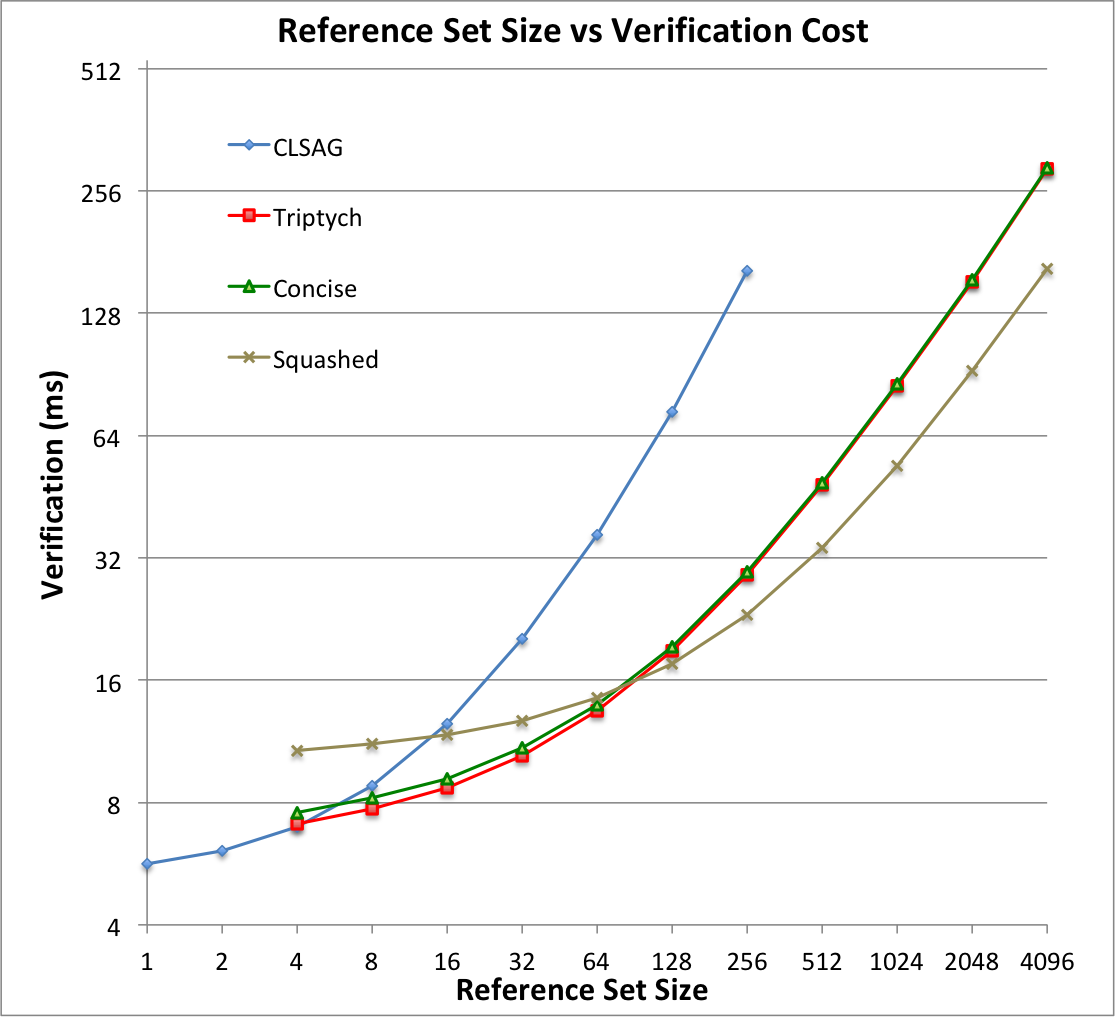
\includegraphics[width=8cm]{figures/refset_1batch_ver.png}
    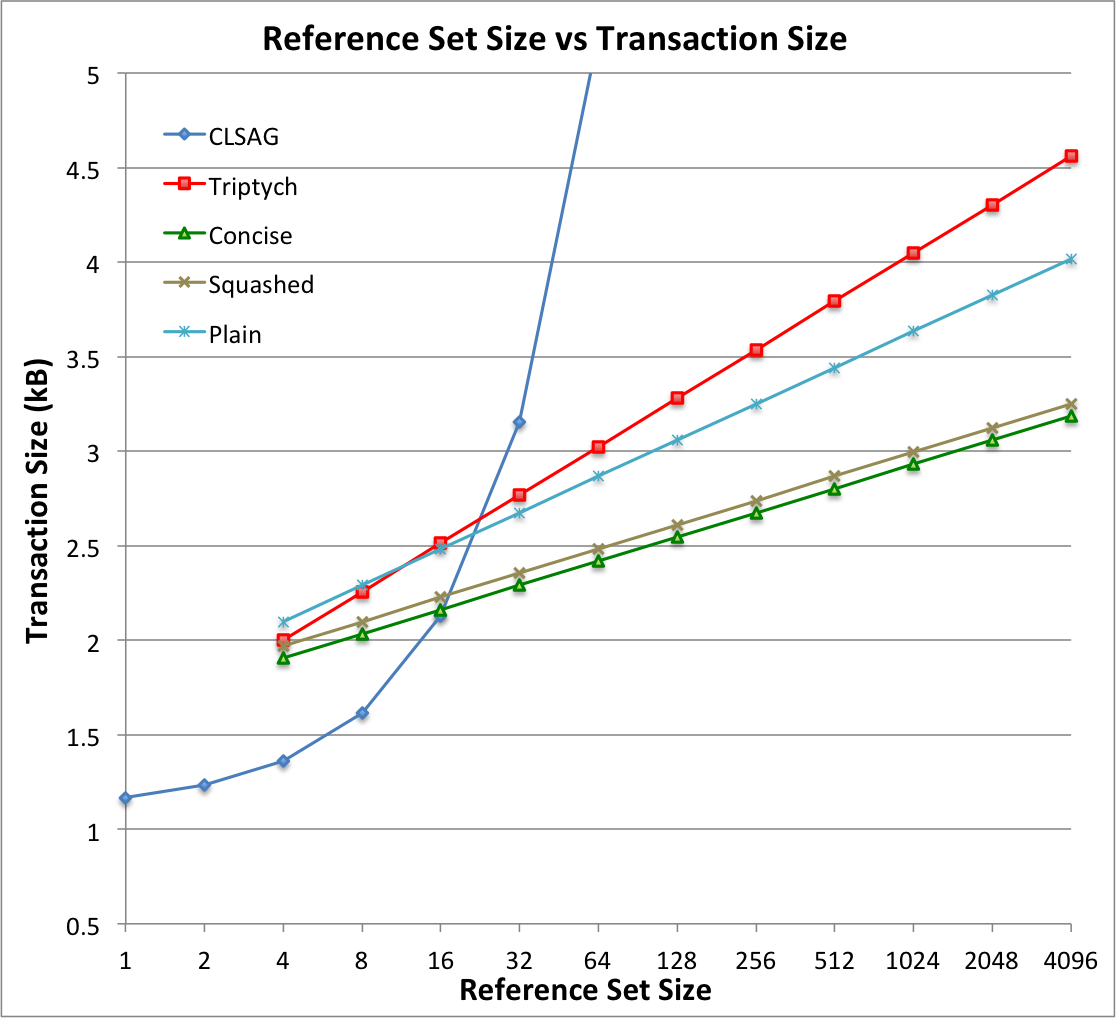
\includegraphics[width=8cm]{figures/refset_1batch_size.png}
    \captionof{figure}{[Left] Membership proof reference set size vs verification cost for 2-input/2-output transactions and no batch-verification. Note that both axes are logarithmic.}
    \label{figure:efficiency-refsetsize-ver}
    \captionof{figure}{[Right] Membership proof reference set size vs verification size for 2-input/2-output transactions and no batch-verification.}
    \label{figure:efficiency-refsetsize-size}
\end{center}

In Figure \ref{figure:efficiency-refsetsize-ver} we see that Seraphis-Concise and Triptych have practically identical verification costs. This is because the modifications to Triptych to get Concise-Grootle proofs have minimal effect on verification costs when reference sizes are reasonably large, and because Seraphis composition proofs have negligible verification cost compared to Concise-Grootle proofs.

Seraphis-Plain is only marginally faster than Seraphis-Concise (less than 10\%), because the verification optimizations that can be used by Seraphis-Plain are relatively inefficient.\footnote{For those readers familiar with Lelantus-Spark's Grootle proofs, we used 2-byte weights to aggregate keys during verification.}

We also see that above reference set size 4, CLSAG performs significantly worse than Seraphis-Concise and Triptych. The performance cost of CLSAG for `large' reference set sizes (above around 5-15) is the driving motivator behind research into protocols like Triptych and Seraphis.

It would seem that Seraphis-Squashed is unfavorable below a reference set size of 128, but Figures \ref{figure:efficiency-refsetsize-ver-25batch} and \ref{figure:efficiency-16inout-ver} will expose the advantages of that protocol variant.

Figure \ref{figure:efficiency-refsetsize-size} further reinforces the costliness of CLSAG, and reveals that Seraphis transaction sizes scale better than Triptych with reference set sizes, which is thanks to the relative simplicity of Concise-Grootle proofs. Here we also see that the marginal performance gains of Seraphis-Plain compared to Seraphis-Concise come at a significant transaction size cost.

\begin{center}
    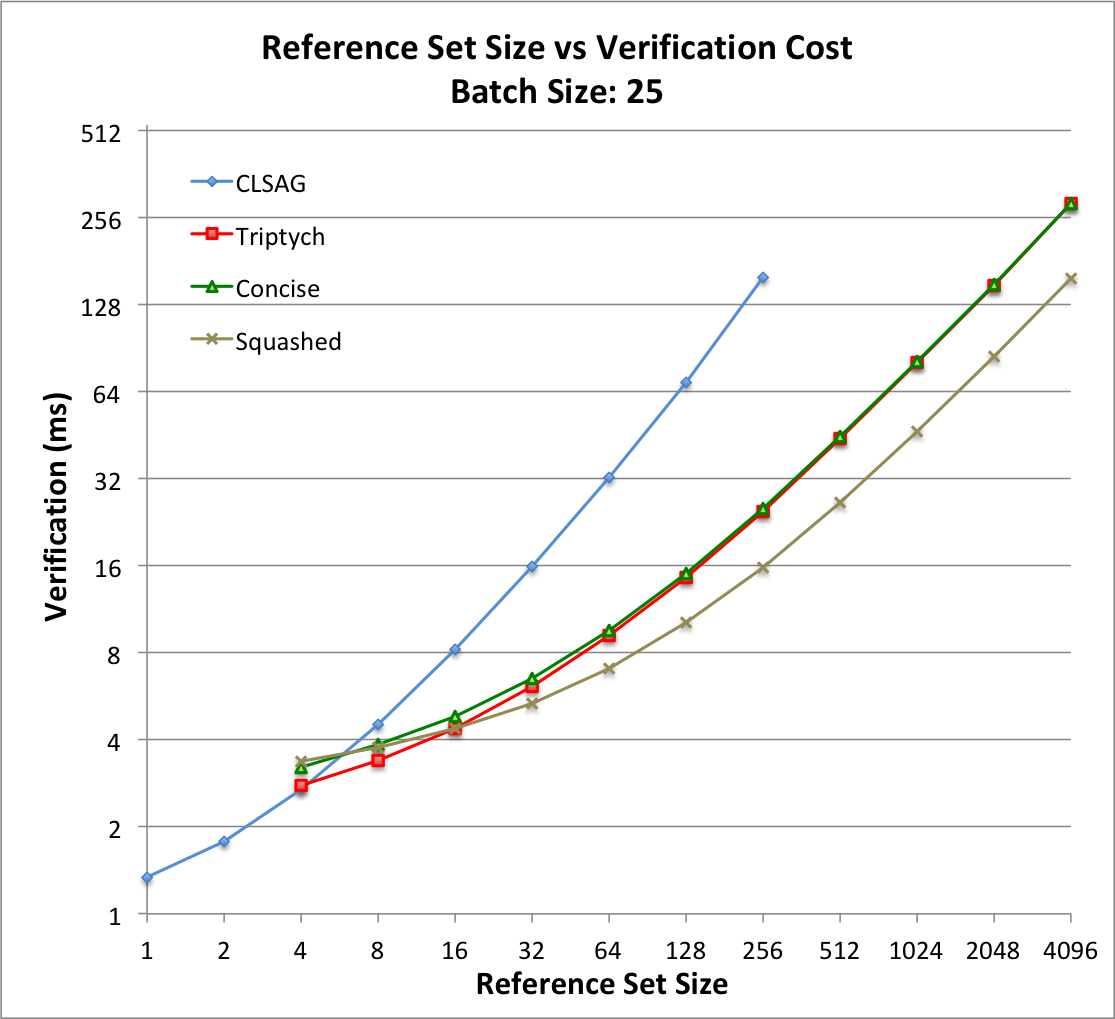
\includegraphics[width=8cm]{figures/refset_25batch_ver.png}
    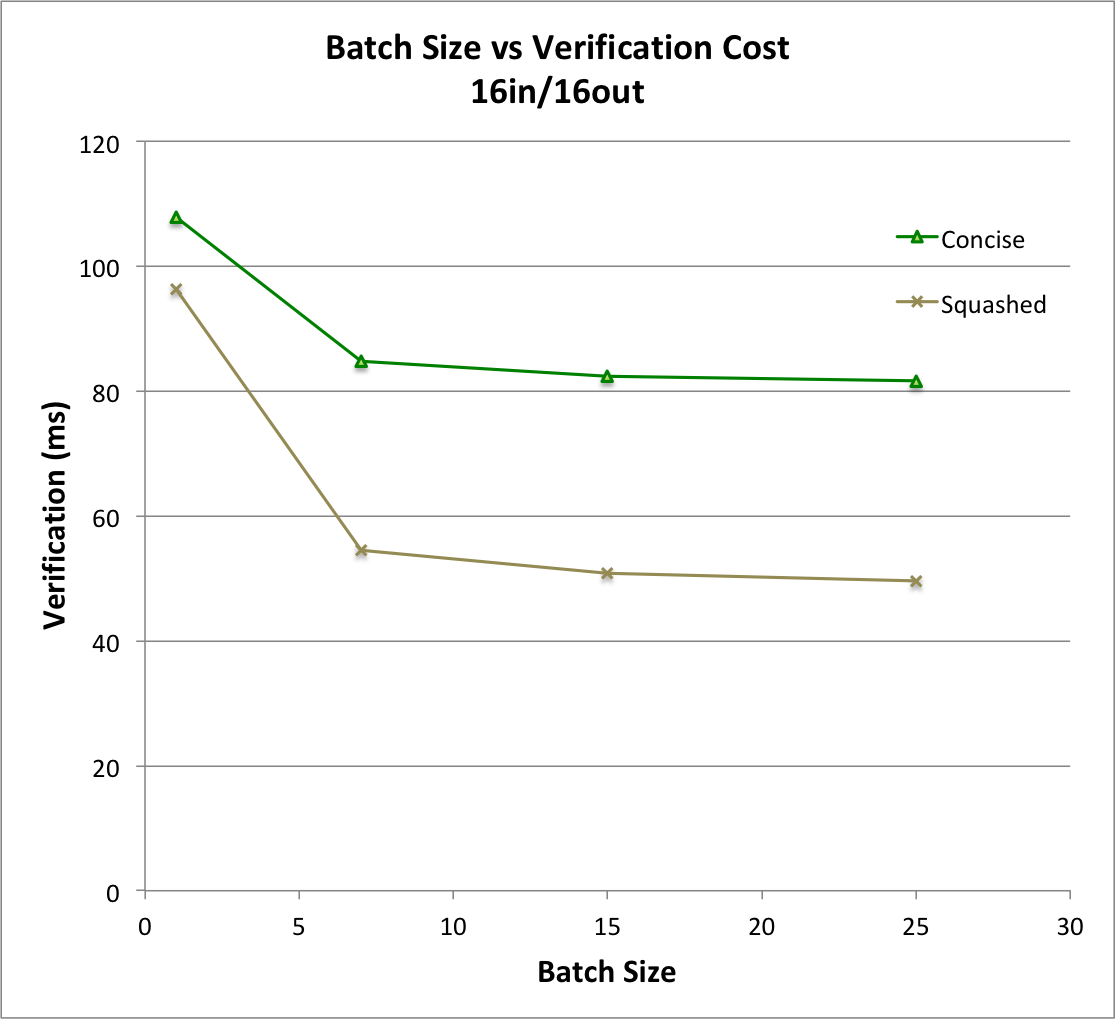
\includegraphics[width=8cm]{figures/16inout_ver.png}
    \captionof{figure}{[Left] Membership proof reference set size vs per-transaction verification cost for 2-input/2-output transactions verified in batches of 25. Note that both axes are logarithmic.}
    \label{figure:efficiency-refsetsize-ver-25batch}
    \captionof{figure}{[Right] Batch size vs per-transaction verification cost for 16-input/16-output transactions with 128-member reference sets.}
    \label{figure:efficiency-16inout-ver}
\end{center}

Figures \ref{figure:efficiency-refsetsize-ver-25batch} and \ref{figure:efficiency-16inout-ver} show what happens when transactions are verified in batches. Multiple Grootle proofs can be verified together in batches, and likewise the aggregated Bulletproofs+ range proofs in a transaction can be batch-verified with range proofs from other equivalent transactions.

Notably, Seraphis-Squashed's performance relative to the other protocols improves greatly when batching is done. This is because Seraphis-Squashed trades simpler membership proofs for range proofs on input image masked amount commitments, and because Bulletproofs+ proofs benefit more from batching than Grootle proofs.\footnote{Grootle proof and Bulletproofs+ proof verification use so-called `multiexponentiation'. It turns out the multiexponentiation operations of those proofs can be combined into one operation, which is a slight optimization (on the order of 1-10\% for unbatched verification).}

\begin{center}
    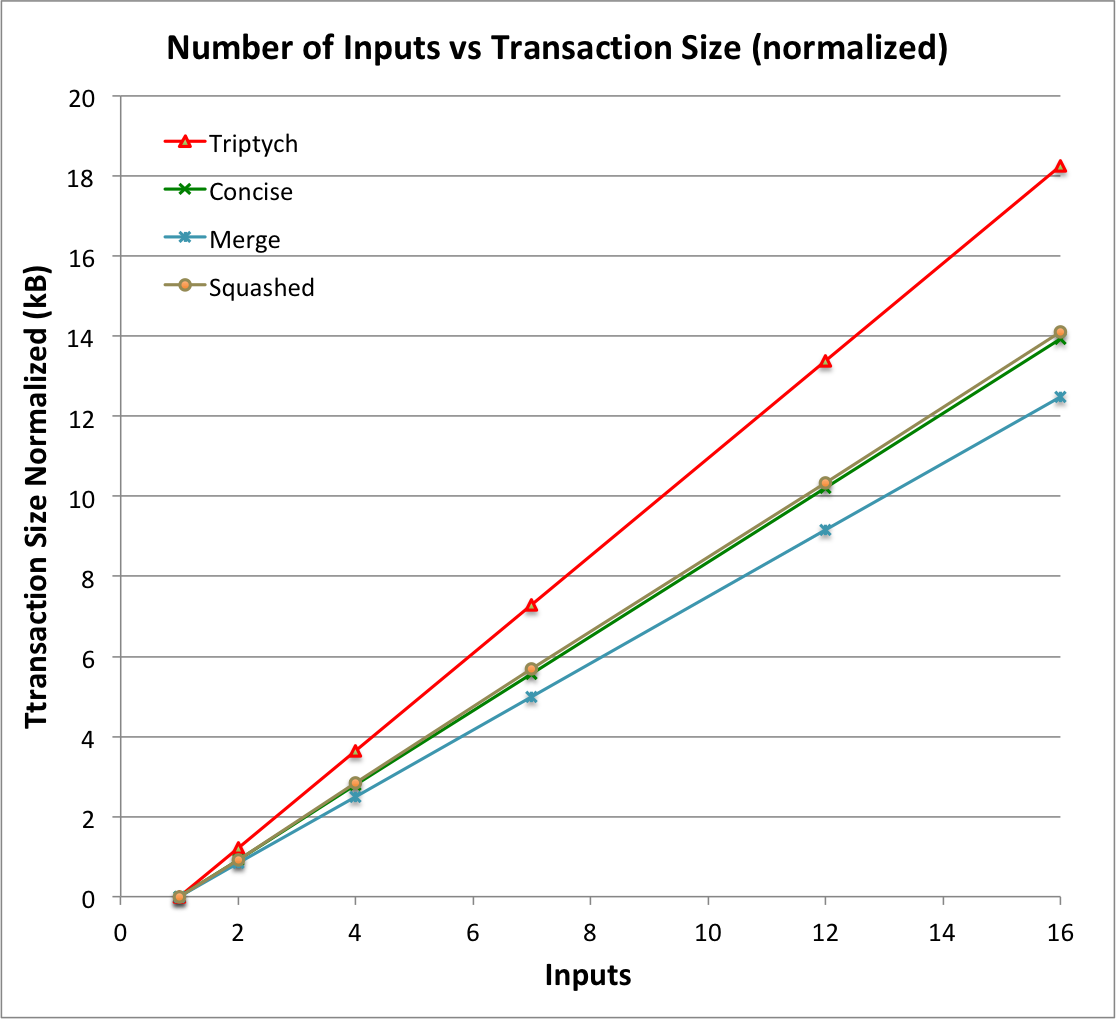
\includegraphics[width=8cm]{figures/inputs_size.png}
    \captionof{figure}{Input count vs transaction size (normalized to the 1-input case) for 2-output transactions with 128-member reference sets and no batch-verification.}
    \label{figure:efficiency-inputs-size}
\end{center}

Finally, in Figure \ref{figure:efficiency-inputs-size} we see how Seraphis-Merge differs from the other variants. In explicit terms, Seraphis-Merge is $32*(1 + 3*(\textrm{num\_inputs} - 1))$ bytes smaller than Seraphis-Concise. Also note that Triptych transaction sizes scale worse with input counts than the Seraphis variants. Even Seraphis-Plain scales better than Triptych with increasing input counts.


% ___________________________________________________________________________________________________________
%
%				BACKMATTER
% ___________________________________________________________________________________________________________

% -------- Bibliography -----------------------

\addcontentsline{toc}{chapter}{Bibliography}
{\footnotesize
\bibliographystyle{plain}
\bibliography{references.bib}
}

% -------- Appendix ---------------------------
\if 11
\newpage
\begin{appendices}

\renewcommand{\theFancyVerbLine}{%
	\textcolor{red}{\small
		\arabic{FancyVerbLine}}}

\section{Squashed e-note model}
\label{appendix:squashed-e-note-model}

The squashed e-note model is a specialization of the Seraphis membership proof model that allows relatively simpler (and more efficient) proof structures.

First we will describe the model, then discuss how it satisfies relevant security requirements when applied to Seraphis.


\subsection{Model}
\label{appendix:squashed-e-note-model-model}

\begin{enumerate}
    \item Let $G_1,...,G_n$ be generators whose discrete logarithm relations with each other, with $G$, and with $H$ are unknown.

    \item Let $\mathbb{S}$ represent a set of tuples $\{K_i, C_i\}$, where\vspace{.115cm}
    \begin{align*}
        K_i &= z_i G + s_{i,1} G_1 + s_{i,2} G_2 + ... + s_{i,n} G_n \\
        C_i &= x_i G + a_{i,1} H
    \end{align*}

    \item Let $\mathbb{S}^t$ represent a set of `transformed' tuples $\{K^t_i, C^t_i\}$, where\vspace{.115cm}
    \begin{align*}
        K^t_i &= \mathcal{H}_6(K_i, C_i)*K_i \\
        C^t_i &= C_i
    \end{align*}

    \item Perform a range proof on each $C^t_i \in \mathbb{S}^t$ (recall Section \ref{subsubsec:confidential-transactions-range-proofs}).

    \item Let $\mathbb{Q}$ represent a set of squashed tuples $\{Q_i\}$, where\vspace{.115cm}
    \[Q_i = K^t_i + C^t_i\]

    \item Let $\tilde{S}$ represent a tuple $\{K', C'\}$, where\vspace{.115cm}
    \begin{align*}
        K' &= z' G + s'_1 G_1 + s'_2 G_2 + ... + s'_n G_n \\
        C' &= x' G + a'_1 H
    \end{align*}

    \item Let $\tilde{Q} = K' + C'$.

    \item Demonstrate that, within a security parameter $k$, $\tilde{Q}$ corresponds to some $Q_{\pi} \in \mathbb{Q}$, where $\pi$ is unknown to the verifier, such that:
    \begin{enumerate}
        \item The discrete log relation of $\tilde{Q} - Q_{\pi} = [(z' + x') - (\mathcal{H}_6(K_{\pi}, C_{\pi})*z_{\pi} + x_{\pi})]*G$ with respect to $G$ is known.
    \end{enumerate}

    \item Perform a range proof on $C'$.

    \item Demonstrate knowledge of $z', s'_1,...,s'_n$ such that $K' = z' G + s'_1 G_1 + s'_2 G_2 + ... + s'_n G_n$.
\end{enumerate}

The benefit of this specialization compared to the underlying membership proof model is you only need to prove the discrete log in one commitment to zero relation, rather than two. For example, with a SAG (e.g.\ LSAG \cite{Liu2004} without linking) or Groth/Bootle one-of-many proof on the set $\{\tilde{Q} - Q\}$. The efficiency implications are discussed in Section \ref{sec:efficiency}, which compares possible instantiations of Seraphis using the two models.


\subsection{Requirement satisfaction}
\label{appendix:squashed-e-note-model-req-satisfaction}

\subsubsection{Underlying membership proof model}

We argue that the squashed e-note model satisfies the underlying membership proof model.

Let $\mathbb{S}^t$ be the input to the underlying model. We will show that the following requirements, adapted from Section \ref{subsec:seraphis-membership proofs}, are met.

\begin{enumerate}
    \item Demonstrate that, within a security parameter $k$, $\tilde{S}$ corresponds to some $S^t_{\pi} \in \mathbb{S}^t$, where $\pi$ is unknown to the verifier, such that:
    \begin{enumerate}
        \item $s'_j == \mathcal{H}_6(K_{\pi}, C_{\pi})*s_{\pi,j}$ for $j \in 1,...,n$
        \item $a'_1 == a_{\pi,1}$
        \item The prover must have knowledge of $\mathcal{H}_6(K_{\pi}, C_{\pi})*z_{\pi}$.
    \end{enumerate}
\end{enumerate}

Observe the following.

\begin{enumerate}
    \item The prover must know $[(z' + x') - (\mathcal{H}_6(K_{\pi}, C_{\pi})*z_{\pi} + x_{\pi})]$ and $z'$ to satisfy the squashed e-note model, and $x'$ and $x_{\pi}$ to construct the range proofs on $C'$ and $C^t_{\pi}$. Therefore the prover must know $\mathcal{H}_6(K_{\pi}, C_{\pi})*z_{\pi}$. The point $\mathcal{H}_6(K_{\pi}, C_{\pi})$ is considered `public knowledge', so the prover must also know $z_{\pi}$.

    \item Range proofing $C_{\pi}$ and $C'$ means they have the form $x G + a H$, implying they contain no $G_1,...,G_n$ components. Therefore, demonstrating discrete log with respect to $G$ in the commitment to zero $\tilde{Q} - Q_{\pi}$ means it must be the case that $s'_j == \mathcal{H}_6(K_{\pi}, C_{\pi})*s_{\pi,j}$ for $j \in 1,...,n$.

    \item Suppose $K_i$ has the form $K_i = z_i G + s_{i,1} G_1 + s_{i,2} G_2 + ... + s_{i,n} G_n + b H$. Since the model demonstrates that $K'$ does not contain any $H$ components, and the commitment to zero $\tilde{Q} - Q_{\pi}$ means all non-$G$ components balance in those two points, it must be the case that $C' = x' G + (a_{i,1} + \mathcal{H}_6(K_{\pi}, C_{\pi})*b)*H$. However, the term $\mathcal{H}_6(K_{\pi}, C_{\pi})$ is both uniformly distributed and implicitly dependent on the values $a_{i,1}$ and $b$, so the value $a'_1 = (a_{i,1} + \mathcal{H}_6(K_{\pi}, C_{\pi})*b)$ will be uniformly distributed in $\mathbb{Z}_l$ (assuming $b$ is non-zero). Since the range proof on $C'$ means that $a'_1$ must be in the range $[0,...,2^z - 1]$, if $b \neq 0$ then the probability that a range proof on $a'_1$ can succeed is $2^z/l$. This means $a'_1 == a_{i,1}$ can be assumed to be true within the security parameter $k$ if $1/k > 2^z/l$.\footnote{Typically $l \approx 2^{252} - 2^{256}$, $2^z = 2^{64}$, and $k = 2^{128}$; $1/2^{128} > 2^{64}/2^{252}$ is true.} [[[formalize better?]]]
\end{enumerate}

\subsubsection{Seraphis structure}

\begin{enumerate}
    \item Note that a range proof on $C_i$ is equivalent to a range proof on $C^t_i$ since $C^t_i = C_i$.

    \item In Seraphis, range proofs on $C_i$ are created when e-notes are first constructed (i.e.\ as outputs of a transaction). This means transaction authors, who reference $C_i$ as part of transaction membership proofs, will not themselves construct range proofs on $C_i$. As a consequence, transaction authors won't necessarily know $x_{\pi}$.

    However, we do not consider this a security problem. When a transaction author sends an e-note to a recipient, they are `delegating spend authority' to that recipient. In the context of membership proofs (i.e.\ step 8 above), any person who knows $(\mathcal{H}_6(K_{\pi}, C_{\pi})*z_{\pi} + x_{\pi})$ must have learned that value by cooperating with the original transaction author. Therefore, whoever constructs a membership proof for an e-note in the above model must be acting as a `proxy' of that e-note's original author. Since the author knows $x_{\pi}$ (recall that they must have range proofed $C_{\pi}$), the value $\mathcal{H}_6(K_{\pi}, C_{\pi})*z_{\pi}$ can be derived from the combined knowledge of the author and his proxy.

    To gain further confidence in this roundabout security proof, consider the following.
    \begin{enumerate}
        \item An e-note's author cannot create a membership proof for that e-note (i.e.\ complete step 8 in the model) unless they know $\mathcal{H}_6(K_{\pi}, C_{\pi})*z_{\pi}$. This trivially follows from the fact they know $x_{\pi}$ as the one who range proved $C_{\pi}$, and they must know $\mathcal{H}_6(K_{\pi}, C_{\pi})*z_{\pi} + x_{\pi}$ as the one who performed step 8 in the above model.

        \item Suppose $p_1 + p_2 = \mathcal{H}_6(K_{\pi}, C_{\pi})*z_{\pi} + x_{\pi}$ ($p_1$ or $p_2$ could be zero). Let the e-note author know $x_{\pi}$ and $p_2$; let the prover of step 8 know $p_1$. In order to complete step 8 from above, the prover must learn $p_2$. Can the prover acquire the pair $p_1, p_2$ without collaborating with someone who knows $x_{\pi}$?

        [[[formal proof? this is giving me a lot of trouble]]]
    \end{enumerate}

    \item Seraphis linking tags are computed from the output of a membership proof, namely the point $K'$ in $\tilde{S}$. However, $K'$ in the squashed e-note model applied to Seraphis has the form $K' = t_k G + \mathcal{H}_6(K^o_{\pi}, C_{\pi})*[k^o_a*U + k^o_b*G]$. This means linking tags will have the form $\tilde{K} = (1/(\mathcal{H}_6(K^o_{\pi}, C_{\pi})*k^o_a))*G$ instead of $\tilde{K} = (1/k^o_a)*G$. Since $\mathcal{H}_6(K^o_{\pi}, C_{\pi})$ is uniquely defined by each e-note (and not malleable), these modified linking tags are also unique per e-note. In other words, only one linking tag can be produced for each e-note in the ledger.

    There is one interesting side-effect. The value $\mathcal{H}_6(K^o_{\pi}, C_{\pi})$ is dependent on the e-note commitment $C_{\pi}$, so it is possible for two e-notes with the same address $K^o$ to produce different linking tags if they have different commitments.

    \item Step 10 in the above model is automatically satisfied by Seraphis because $K'$ is passed as input to the ownership/unspentness proof system, which demonstrates knowledge of the per-generator discrete log relations of its inputs.
\end{enumerate}


\subsection{Practical considerations}
\label{appendix:squashed-e-note-model-practical-considerations}

\begin{enumerate}
    \item Transaction verifiers can pre-compute steps 3 and 5 from the above model for every e-note in the ledger. The squashed tuples $Q_i$ can be stored in anticipation of new transactions that may require them.

    \item In transaction chaining (Section \ref{subsec:implementers-other-recommendations}), only step 8 in the above model needs to be deferred (assuming $Q_i$ values have been precomputed, and range proofs on $C_i$ already exist).
\end{enumerate}



\section{Generalized Schnorr signatures}
\label{appendix:generalized-schnorr-signatures}

- generalized Schnorr signature
    - signing with multiple private keys in parallel (shared challenge)
    - concise aggregation on common base points (compressing private keys)
    - multi-base signing (same DL across multiple bases)



\section{Groth/Bootle one-of-many proofs}
\label{appendix:grootle-one-of-many-proofs}

- Grootle (parallel vs non-parallel)



\end{appendices}
\fi
% -------- Last page -------------------------



\end{document}